% Contributions are much appreciated, in order to contribute to this project, head over to this repository:
% https://github.com/bshramin/uofa-eng-assignment

\documentclass[11pt,letterpaper]{article}
\textwidth 6.5in
\textheight 9.in
\oddsidemargin 0in
\headheight 0in
\usepackage{graphicx}
\usepackage{fancybox}
\usepackage[utf8]{inputenc}
\usepackage{epsfig,graphicx}
\usepackage{multicol,pst-plot}
\usepackage{pstricks}
\usepackage{amsmath}
\usepackage{amsfonts}
\usepackage{amssymb}
\usepackage{eucal}
\usepackage[left=2cm,right=2cm,top=2cm,bottom=2cm]{geometry}
\usepackage{esvect}
\pagestyle{empty}
\DeclareMathOperator{\tr}{Tr}
\newcommand*{\op}[1]{\check{\mathbf#1}}
\newcommand{\bra}[1]{\langle #1 |}
\newcommand{\ket}[1]{| #1 \rangle}
\newcommand{\braket}[2]{\langle #1 | #2 \rangle}
\newcommand{\mean}[1]{\langle #1 \rangle}
\newcommand{\opvec}[1]{\check{\vec #1}}
\renewcommand{\sp}[1]{$${\begin{split}#1\end{split}}$$}

\usepackage{lipsum}

\usepackage{listings}
\usepackage{color}
\usepackage{wrapfig}
\usepackage[shortlabels]{enumitem}

\definecolor{codegreen}{rgb}{0,0.6,0}
\definecolor{codegray}{rgb}{0.5,0.5,0.5}
\definecolor{codepurple}{rgb}{0.58,0,0.82}
\definecolor{backcolour}{rgb}{0.95,0.95,0.92}

\lstdefinestyle{mystyle}{
	backgroundcolor=\color{backcolour},   
	commentstyle=\color{codegreen},
	keywordstyle=\color{magenta},
	numberstyle=\tiny\color{codegray},
	stringstyle=\color{codepurple},
	basicstyle=\footnotesize,
	breakatwhitespace=false,         
	breaklines=true,                 
	captionpos=b,                    
	keepspaces=true,                 
	numbers=left,                    
	numbersep=5pt,                  
	showspaces=false,                
	showstringspaces=false,
	showtabs=false,                  
	tabsize=2
}

\lstset{style=mystyle}

\begin{document}
\pagestyle{plain}

\begin{flushleft}
Estudiante: Fabio Quimbay\\
Email: fabio.quimbay883@comunidadunir.net\\
Profesor: Miguel Ángel Cabeza\\
Fecha: Noviembre 13 de 2022\\
\end{flushleft}

\begin{flushright}\vspace{-20mm}

\includegraphics[height=2cm]{logo.png}
\end{flushright}
 
\begin{center}\vspace{0cm}
\textbf{\large PER5786 2022-2023  Física 1 (GFI) - PER5786 2022-2023}\\
 Tema 3 - Movimientos elementales
\end{center}

 
\rule{\linewidth}{0.1mm}
%%%%%%%%%%%%%%%%%%%%%%%%%%%%%%%%%%%%%%%%%%%%%%%%%%%%%%%%%%%%%%%%%%%%%%%%

\bigskip
\bigskip

%%%%%%%%%%%%%%%%%%%%
\textbf{Problema propuesto 7}\\

A. Sabiendo que el radio terrestre es $R= 6378.137\,k$. y un día sidéreo son 23 horas, 56 minutos, y 4'091 segundos, calcula para un punto de la tierra con latitud L la magnitud de la velocidad lineal de las siguientes ubicaciones:

\begin{enumerate}
  \item Cosmódromo Ruso de Baikonur, $L =45'920^{\circ}\,N$.
  \item Estación de lanzamiento de la NASA en Cabo Cañaveral, EE.UU., $L =28'394^{\circ}\,N$.
  \item Estación de lanzamiento de la ESA en la Guayana Francesa, $L=5'167^{\circ}\,N$.
\end{enumerate}

Razona desde cuál de estas 3 ubicaciones preferirías lanzar un cohete al espacio para enviar un satélite a una órbita ecuatorial geoestacionaria.\\

B. Si un avión MiG-25 despega desde Baikonur con una velocidad Mach $3.2\,(Mach\,1 = 343\,m/s)$ hacia el este, ¿medirá $9,8\,m/s^2$ su acelerómetro hacia el centro de la tierra?\\

\begin{wrapfigure}{r}{0.25\textwidth}
\begin{center}
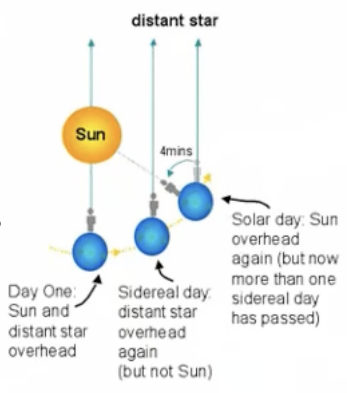
\includegraphics[width=0.25\textwidth]{problema_7.png}
\end{center}
\end{wrapfigure}

\textbf{Formulas base:}\\

Se tomarán las siguientes formulas base del MCUA:

\begin{align}
\boxed{ \vec{a_{c}} = \frac{v^2}{r} = \frac{(w \cdot r)^2}{r} = w^2 \cdot r}\\
\boxed{ T = \frac{2\pi}{\omega}}\\
\boxed{ cos \lambda = \frac{R}{R_{T}}}\\
\boxed{ V = \omega \cdot r = \omega \cdot R \cdot cos \lambda}
\end{align}

\textbf{Solución:}\\

Establecemos algunas magnitudes, para que sean correspondientes al SI, a saber:

\begin{align*}
R = 6378.137\,k = 6378138\,m\\
T = 23\,h\,56\,m\,4.091\,s \approx 86164\,s\\
\end{align*}

Ahora determinamos la velocidad angular de acuerdo al periodo dado:

\begin{align}
\omega &= \frac{2 \cdot \pi}{T} = \frac{2 \cdot \pi}{86164} = 0.000072921 \approx 7.2921 \times 10^{-5} 
\end{align}

Ahora se establecen las diferentes velocidades lineales para cada uno de puntos de lanzamiento:

\begin{align}
V_{A} &= 7.2921 \times 10^{-5} \cdot 6378137 \cdot cos\,45.920 ^{\circ} = 323.553\,m/s\\
V_{B} &= 7.2921 \times 10^{-5} \cdot 6378137 \cdot cos\,28.394 ^{\circ} = 409.148\,m/s\\
V_{C} &= 7.2921 \times 10^{-5} \cdot 6378137 \cdot cos\,5.1670 ^{\circ} = 463.21\,m/s
\end{align}

Posteriormente, es necesario calcular la velocidad lineal del avión, a saber:

\begin{align}
V_{L_{AVION}} = 3.2 \times 343\,m/s = 1097.6\,m/s
\end{align}

Con la información obtenida, procedemos a encontrar la aceleración normal de cada punto de lanzamiento, con el propósito de determinar la que mayor aceleración provea, a saber:

\begin{align}
a_{N_{A}} = \frac{V_{L}}{r} = \frac{V_{L}}{R_{T} \cdot cos \lambda} = \frac{323.553^2}{6378137 \cdot 45.920^{\circ}} = 0.023594\,m/s^2\\
a_{N_{B}} = \frac{V_{L}}{r} = \frac{V_{L}}{R_{T} \cdot cos \lambda} = \frac{409.148^2}{6378137 \cdot 28.394^{\circ}} = 0.029835\,m/s^2\\
a_{N_{C}} = \frac{V_{L}}{r} = \frac{V_{L}}{R_{T} \cdot cos \lambda} = \frac{463.21^2}{6378137 \cdot 5.167^{\circ}} = 0.033778\,m/s^2
\end{align}

De tal manera que el punto de lanzamiento de la ESA ubicado en la Guyana Francesa es el ideal para enviar un satélite a una órbita ecuatorial geoestacionaria, dado que provee un mayor aceleración, lo que permitirá que el cohete arribe en menor tiempo.\\

Para poder determinar si el avión MiG-25 bajo las condiciones descritas, tendrá una aceleración igual a $9.8\,m/s^2$ es necesario tomar como referencia la velocidad lineal del avión ($1097.6\,m/s$) y calcular la aceleración nominal, a saber:

\begin{align}
a_{N_{AVION}} &= \frac{V^2_{AVION}}{R_{Baikonur}} = \frac{1097.6^2}{R_{T} \cdot cos \lambda} = \frac{1097.6^2}{6378137 \cdot cos 45.920^{\circ}} = 0.271516\,m/s
\end{align}

Con la aceleración normal calculada en ese punto, procedemos a determinar que tanto se ve afectada la aceleración de la gravedad:

\begin{align}
\vec{a} = \vec{a_{c}} - g = 0.271516 - 9.8 = 9.52848\,m/s^2
\end{align}

Por lo que podemos concluir que la gravedad en el punto de Baikonur será de $9.52848\,m/s^2$.

%%%%%%%%%%%%%%%%%%%%

\end{document}

